\documentclass[12pt]{article}
\usepackage[T1]{fontenc}
%\usepackage[latin9]{inputenc}
\usepackage[utf8]{inputenc}
\usepackage[english]{babel}
\usepackage{amsmath}
\usepackage{amsfonts}
\usepackage{amssymb}
\usepackage{setspace}
\usepackage{rotating}
\usepackage{graphics}
\usepackage[round]{natbib}
\usepackage{graphicx}
\usepackage{float} 				%allows you to float images
\usepackage{latexsym}
\usepackage{bbding}
\usepackage {moresize}
\usepackage{bbding}
\usepackage{blindtext}
\usepackage{hhline}
\usepackage{tikz}
\usetikzlibrary{shapes,backgrounds}
\usepackage{pgfplots}
\usetikzlibrary{arrows}
\usepackage{enumitem}
\doublespacing
\usepackage{geometry}
\usepackage{amsthm}
\usepackage{color}
\usepackage{array,multirow}
\usepackage{subcaption}
\usepackage{pst-plot}
	\psset{xunit=15mm}
\geometry{verbose,tmargin=1in,bmargin=1in,lmargin=1in,rmargin=1in}
\setlength{\parskip}{\bigskipamount}
\setlength{\parindent}{0pt}

\newenvironment{problem}[2][Problem]{\begin{trivlist}
\item[\hskip \labelsep {\bfseries #1}\hskip \labelsep {\bfseries #2.}]}{\end{trivlist}}

\title{Problem Set 1 \thanks{Problem list - 2.2.4, 2.2.28, 2.3.2, 2.3.16, 2.4.23, 2.5.16}}
\author{Ian McGroarty \\
	Course Number: 625.603}
\date{February 7, 2019}

\begin{document}

\maketitle

\begin{problem}{2.2.4} Let A be the event that the sum of two cards is 8 (assume that aces have numerical value of one). How many outcomes are in A? \\
\textbf{Solution:} \underline{54 total outcomes in A.}  \\
\textbf{Explanation}
To answer this question we must first see how many ways can we express 8 as the sum of 2 natural numbers -  {(1,7),(2,6),(3,5),(4,4)}. Note that since we only care that the sum is equal to 8, the order does not matter. Since you can have the ace of hearts, the ace of spades, the ace of diamonds, the ace of clubs there are 4 cards of the 52 to represent any one number. There are 16 possible combinations of cards that could make result in a (1,7) combination as seen by the matrix below, where $A_h$ represents the Ace of hearts and $7_d$ represents the 7 of diamonds, ect.: 
$$
\begin{bmatrix}
(A_h,7_h) & (A_d,7_h) & (A_c,7_h) & (A_s,7_s) \\
(A_h,7_d) & (A_d,7_d) & (A_c,7_d) & (A_s,7_d) \\
(A_h,7_c) & (A_d,7_c) & (A_c,7_c) & (A_s,7_c) \\
(A_h,7_s) & (A_d,7_s) & (A_c,7_s) & (A_s,7_s) 
\end{bmatrix}
$$
By symmetry,  (2,6) and (3,5) will also each have 16 combinations. Bringing the total to 16*3=48. Since (4,4) involves the same number card the pulling the 4 of hearts means that you can only pull the 4 of clubs also. This can be expressed as ``4 choose 2``. If necessary the formula $\frac{n!}{k!(n-k)!}$ can be applied, where n=4 and k=2. This shows us that there are 6 combinations, listed in the matrix below: 
$$
\begin{bmatrix}
(4_h,4_d) & (4_d,4_c) & (4_c,4_s) \\
(4_h,4_c) & (4_d,4_s) & \\
(4_h,4_s) &  & 
\end{bmatrix}
$$
Adding together our combinations 48+6= \underline{54 total outcomes in A.}
% \\
%Set $A =( P(1)\cap P(2)$ ) \\
%The probability of drawing an ace with value 1 is $\frac{4}{52}$ \\
\end{problem}


\begin{problem}{2.2.28}
\begin{align*}
S &= {x:0\leq x \leq 10} \\
A &= {x:0<x<5} \\
B &= {x: 3\leq x\leq 7}\\
\end{align*}


\textbf{Work:} Let's draw a number line:

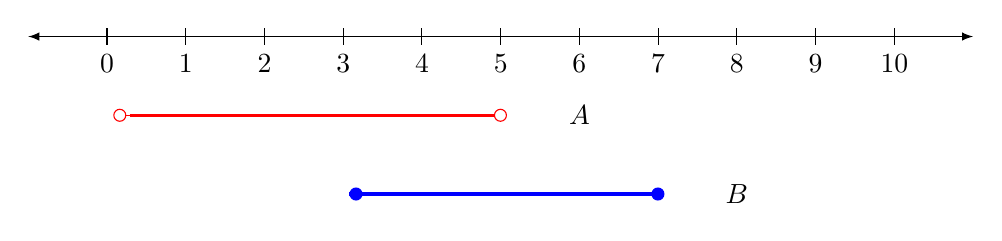
\begin{tikzpicture}
\draw[latex-latex] (-1,0) -- (11,0) ; 	%edit here for the axis
\foreach \x in  {0,1,2,3,4,5,6,7,8,9,10} 		% edit here for the vertical lines
\draw[shift={(\x,0)},color=black] (0pt,3pt) -- (0pt,-3pt);
\foreach \x in {0,1,2,3,4,5,6,7,8,9,10} % edit here for the numbers
\draw[shift={(\x,0)},color=black] (0pt,0pt) -- (0pt,-3pt) node[below] 
{$\x$};

\draw[o-o,color=red] (0.08,-1) -- (5.08,-1);
\draw[very thick,color=red] (0.29,-1) -- (4.92,-1);
\node at (6,-1) {$A$};

\draw[*-*,color=blue] (3.08,-2) -- (7.08,-2);
\draw[very thick,color=blue] (3.08,-2) -- (7.08,-2);
\node at (8,-2) {$B$};
\end{tikzpicture}
\\
\textbf{Solutions:} Where ``[" indicates a closed bracket (inclusive) and ``(" indicates open bracket (non-inclusive).\\
\textbf{(a)} $A^c$ = $[0] \cup [5,10] $\\
\textbf{(b)} $A \cap B $ = $[3,5)$ \\
\textbf{(c)} $A \cup B $ = $(0,7]$ \\
\textbf{(d)} $A \cap B^C$ = $[0,3]$  \\
\textbf{(e)} $A^C \cup B$ = $[0] \cup [3,10]$\\
\textbf{(f)} $A^C \cap B^C$ = $[0] \cup (7,10]$
\end{problem}

\begin{problem}{2.3.2} 
P(A) = 0.4, P(B) = 0.5, and P(A $\cap $ B) = 0.1. What is the probability that A or B will occur but not both. \\

%%%% VENN DIAGRAM
\def\firstcircle{(0,0) circle (3)}
\def\secondcircle{(45:4cm) circle (3)}

\begin{tikzpicture}
    \draw \firstcircle node[below] {$A=0.4$};
    \draw \secondcircle node [above] {$B=0.5$};
 \node at (45:2)    {$A \cap B$=0.1};
\end{tikzpicture}
\\
\\
\\
\textbf{Solution:} $P(A^C \cap B) \cup (B^C \cap A)$ = 0.7. Work shown below:
\begin{align*}
P(A^C \cap B)  \cup (B^C \cap A) &= \\
&=P(B) - P(A \cap B)  + P(A) - P(A \cap B) \\
&=P(B) + P(A) + 2P(A \cap B) \\
&=0.5 + 0.4 + 2(0.1)  = 0.7 \\
\end{align*}
\end{problem}

\begin{problem}{2.3.16} Let A be the event that the sum of the two faces showing is 6. Let B be the event that the face showing on one die is twice the face showing on the other. Calculate $P(A \cap B^C)$. \\

\textbf{Solution:} $(A\cap B^C) = \frac{3}{1296} $ \\
 Let's define $B^C$ as the event that the face showing on one die is NOT twice the face showing on the other. Thus, $P(A \cap B^C)$ is the probability that BOTH the dice add up to 6 AND the value of one die is NOT twice the value of the other die: 
\begin{align*}
 A &= \{(1,5),(2,4),(3,3)\} \\
B &= \{(1,2),(2,4),(3,6)\} 
%A \cup B &= \{(1,2),(1,5),(2,4),(3,3),(3,6)\} 
\end{align*}
%We can see right away that $(A\cap B) = \{(2,4)\}$.We know that:
We can see right away that $(A\cap B^C) =  \{(1,5),(3,3)\}$. Since order does not matter in this case we have $(A\cap B^C) =  \{(1,5),(5,1),(3,3)\}$. The two dice are independent, and by independence -  $P(A\cap B) = P(A)\cdot P(B)$ We also can see the the rolls are mutually exclusive, by Axiom 3 - $P(A\cup B)=P(A)+P(B)$. Simply: 
\begin{align*}
P(A\cap B^C) &=P( \{(1,5),(5,1),(3,3)\}) \\
&= P(1,5) \cup P(5,1) \cup P(3,3) && \text{Union (pg20)} \\
&= P(1 \cap 5) \cup P(5 \cap 1) \cup P(3 \cap 3) && \text{Intersection (pg 20)} \\
&= P(1)*P(5) \cup P(5)*P(1) \cup P(3)*P(3) && \text{Independence (pg 50)} \\
&= P(1)*P(5) + P(5)*P(1) + P(3)*P(3) && \text{Axiom 3 (pg 26)} \\
&= (\frac{1}{36}*\frac{1}{36}) + (\frac{1}{36}*\frac{1}{36}) + (\frac{1}{36}*\frac{1}{36}) \\
&= \frac{3}{1296}
\end{align*}
\\
\end{problem}



\begin{problem}{2.4.23} Need to win at least 2 to play. Probabilities of winning each of their last four games are 0.60, 0.50, 0.40, and 0.70 respectively.\\
\textbf{(a)} 0.766 \\
I've grown lazy with my explanations. Let me know if this isn't detailed enough so I know what to do for future problem sets! I've written out each possible combination of wins and losses and their corresponding probabilities in an excel table. Which I've included below (Figure 1), it includes each scenario in which the team wins at least 2 games, and the corresponding probability of the win/loss. The last column is the product of the probabilities, which we can do by the independence of each game. I then sum together the events, allowed by axiom 3 since they are mutually exclusive. The bottom leftmost cell contains this sum.\\
\textbf{(b)} No. Though, I must admit this question is confusing, I had to read it a few times, but I guess that is the idea. Point is that the question is asking if $$P(G4=W) = P(G_N=W | G_X=G_Y=G_Z=W \text{ s.t }(N \neq X \neq Y \neq Z))$$ This does not lend itself to be equal to the question posed in \textbf{(c)} unless the $G_X,G_Y,G_Z$ are the first three games. \\
\textbf{(c)} Yes. Since the games are independent, P(G4=W | G1=G2=G3 = W) = P(G4) by the definition of independence (pg 50). Since the first three games have already been won, a fourth game win guarantees a four game win streak.  

\end{problem}




\begin{problem}{2.5.16} First and second light are green for 40 seconds / minute. The third and fourth are green for 30 seconds/minute. What is the probability that the commuter has to stop at least 3 times. \\
\textbf{Solution:} The probabilities that $L_1$ \& $L_2$ are red are 2/6, or 0.33 each.  The probabilities that $L_3$ \& $L_3$ are red are 3/6, or 0.5 each. Let $L = \{L_1,L_2,L_3,L_4\}$ be the set of lights such that at least 3 are red. 
$$ L = \{(R,R,R,R),(R,R,R,G),(R,R,G,R),(R,G,R,R),(G,R,R,R)\} $$ 
Since the lights are independent and the events are mutually exclusive, we can express the probabilities as: 
$$ (P(L_{1R}) \cap P(L_{2R}) \cap P(L_{3R}) \cap P(L_{4R})) \cup ... \cup (P(L_{1G}) \cap P(L_{2R}) \cap P(L_{3R}) \cap P(L_{4R}))$$
$$ (P(L_{1R}) * P(L_{2R}) * P(L_{3R}) * P(L_{4R})) + ... + (P(L_{1G}) * P(L_{2R}) * P(L_{3R}) * P(L_{4R}))$$
I again just used excel to make the calculations: The table is included below (Figure 2). 

\begin{figure}[h!]
  \includegraphics[width=\linewidth]{2-4-23.png}
  \caption{Excel table for 2-4-23}
  \label{fig:boat1}
\end{figure}

\begin{figure}[h!]
  \includegraphics[width=\linewidth]{2-5-16.png}
  \caption{Excel table for 2-5-16}
  \label{fig:boat1}
\end{figure}

\end{problem}


\end{document}




















%%%%%%%%%%%%%%%%%%%%%%%%%%%%%%%%%%%%%%%%%%%%%%%%%%%%%%%%%%%%%%%%%%%%%%%%%%%%%
%%%%%%%%%%%%%%%%%%%%%%%%%%%%%%%%%%%%%%%%%%%%%%%%%%%%%%%%%%%%%%%%%%%%%%%%%%%%%
%%%%%%%%%%%%%%%%%%%%%%%%%%%%%%%%%%%%%%%%%%%%%%%%%%%%%%%%%%%%%%%%%%%%%%%%%%%%%
%%%%%%%%%%%%%%%%%%%%%%%%%%%%%%%%%%%%%%%%%%%%%%%%%%%%%%%%%%%%%%%%%%%%%%%%%%%%%%%%%%%%%%%%%%%%%%%%%%%%%%%%%%%%%%%%%%%%%%%%%%%%%%%%%%%%%%%%%%%%%%%%%%%%%%%%%%


\begin{align*}
 P(A) &= P(A \cap B) + P(A\cap B^C) && \text{Axiom 3} \\
P(A) - P(A \cap B) &= P(A\cap B^C)  \\
 2*((\frac{1}{36}*\frac{1}{36}) + (\frac{1}{36}*\frac{1}{36}) + (\frac{1}{36}*\frac{1}{36})) - 2*((\frac{1}{36}*\frac{1}{36})) &= P(A\cap B^C) && \text{*2 for both die}\\
\\
\frac{4}{1296} &= (A\cap B^C) 
\end{align*}

\begin{align*}
S=&\{0,1,2,3,4,5,6,7,8,9,10\} \\
A = &\{1,2,3,4\} \\
B = &\{3,4,5,6,7\} 
\end{align*}

problem 1
\textbf{Note:} This can be expressed more easily using the probability function: Let $\alpha_i $ be the event that card $i$ is pulled. We want to know: 

\begin{align} 
(\alpha_{ace} \cap \alpha_7) \cup (\alpha_2 \cap \alpha_6) \cup & (\alpha_3 \cap \alpha_5) \cup (\alpha_4 \cap \alpha_4) && \\
(\alpha_{ace} \cap \alpha_7) + (\alpha_2 \cap \alpha_6) +  & (\alpha_3 \cap \alpha_5) + (\alpha_4 \cap \alpha_4) &&\text{ Mutually exclusive events} \\
(\alpha_{ace}* \alpha_7) + (\alpha_2 *\alpha_6) +  & (\alpha_3 *\alpha_5) + (\alpha_4 \cap \alpha_4) &&\text{Independence}
\end{align}



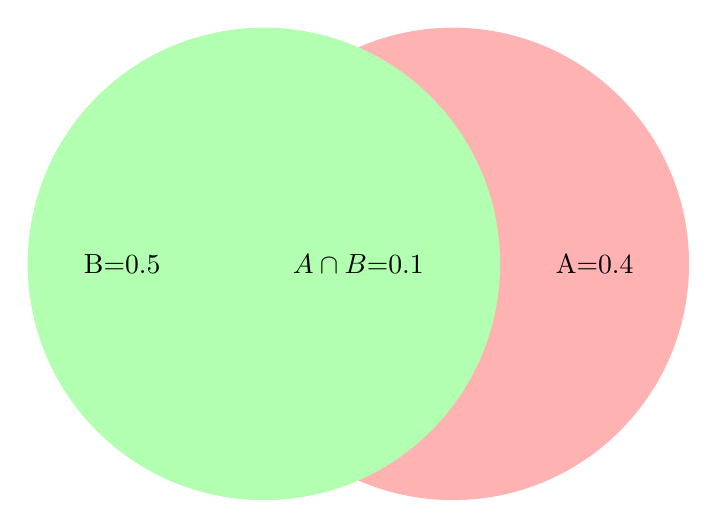
\begin{tikzpicture}
\begin{scope} [fill = gray!50, gray!50];
 \fill[red!30!white]   (0:1.2) circle (3);
    \fill[green!30!white] (180:1.2) circle (3);
\end{scope}
 \node at ( 0:3)    {A=0.4};
  \node at (180:3)    {B=0.5};
  \node at (180:0)    {$A \cap B$=0.1};


\end{tikzpicture}

Two win 2 it is: 
$$P(G1 \cap G2) \cup P(G1 \cap G3) \cup P(G1 \cap G4) \cup P(G2 \cap G3) \cup P(G2 \cap G4) \cup P(G3 \cap G4) $$
Using the general multiplication rule, and because these games are independent events, we can 